\documentclass[12pt]{article}
\usepackage{graphicx}
\usepackage[british,UKenglish,USenglish,english,american]{babel}
\usepackage{tocbibind}
\usepackage[toc,page]{appendix}

%--------------dodatkowe pakiety:-----------
\usepackage{mathtools}
\usepackage{amsfonts}
\usepackage{amsmath}
\usepackage{amsthm}
\usepackage{array}
% for code snippets:
\usepackage{listings}
% for plots:
\usepackage{pgfplots}
\pgfplotsset{width=11cm,compat=1.9}
%-------------------links------------------
\usepackage{hyperref}
\hypersetup{
    colorlinks=true,
    linkcolor=blue,
    filecolor=magenta,      
    urlcolor=cyan,
}
 
\urlstyle{same}
%------placing image caption at the bottom---------
\usepackage{floatrow}
%--------------allows pic alligning----------------
\usepackage[export]{adjustbox}
%---------------------plot3d--------------------------
\usepackage{pgfplots}
\begin{document}

\title{Introduction to CUDA and OpenCL}
\author{Ilona Tomkowicz, Zofia Pieńkowska}

\maketitle
\tableofcontents
\newpage
%--------------------------------------------------------------------

\section{Communication with GPU} \label{gpu_communication}

In order to check details about the GPU used by VM on labolatories (GeForce GTX 1060 6GB) we used a template project deviceQuery.

\subsection{How to establish connection with device} \label{ht_open_connection}
To etract information about the devices connected to host we use funcion
\begin{lstlisting}[language=C]
cudaGetDeviceCount(&deviceCount)
\end{lstlisting} cudaGetDeviceCount(\&deviceCount), which returnes the flag message and changed the passed argument according to the number of devices that were found. Setting onection is done by calling:
\begin{lstlisting}[language=C]
cudaSetDevice(dev_index);
\end{lstlisting}
Where dev\_index is the index of GPU found (for only 1 GPU it will be 0).

\subsection{How to fetch information about GPU} \label{fetch_info}
To fetch information about GPU, after completing steps in previous point, we can call:
\begin{lstlisting}[language=C]
cudaDeviceProp deviceProp;
cudaGetDeviceProperties(&deviceProp, dev_index).
\end{lstlisting}
to get information about device properties or 
\begin{lstlisting}[language=C]
cudaDriverGetVersion(&driverVersion);
cudaRuntimeGetVersion(&runtimeVersion);
\end{lstlisting}
to check driver and runtime version.
After that we can extract specific data like memory size, clock rate, etc using these functions parameters.

\section{Experiments with data size and grid layout}  \label{experients}
Experiments with performance were made using template vectorAdd. This template originally
\begin{itemize}
\item allocates memory in host and device,
\item copies the host input vectors A and B into device memory,
\item sets grid layout,
\item uses created kernel to make caculations,
\item copies the result back into host,
\item veifies if the result is correct
\item frees memory on both, device and host.
\end{itemize} 
The thread size can change up to 1024, larger threads cannot be built and an error is thrown.

\subsection{Computation time comparison}  \label{size_tests}

For fixed vector size $2^{27}$ and changing grid layout, where blocks and threads size are in a relation with each other in following experiments (changing thread number changes blocks number). 
\[ blocksPerGrid =  (vectorElemNumber + threadsPerBlock + 1) / threadsPerBlock \]

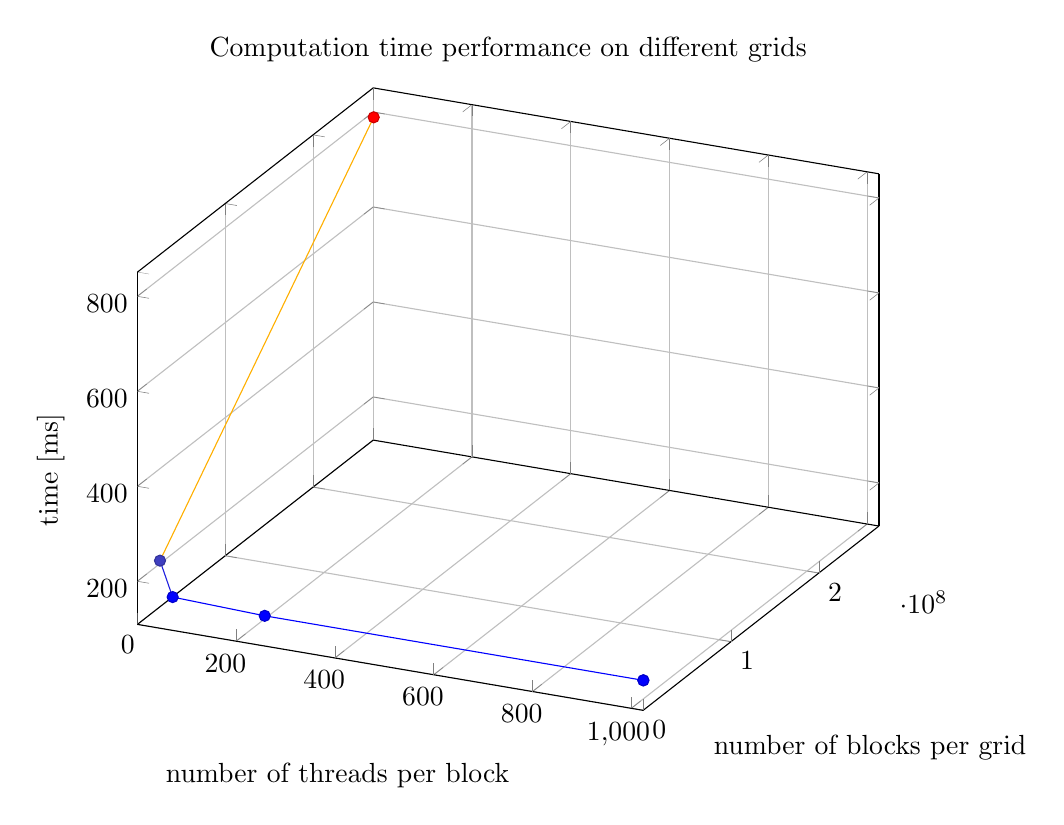
\begin{tikzpicture}
	\begin{axis}[grid=major,
	title={Computation time performance on different grids},
	xlabel={number of threads per block},
	ylabel={number of blocks per grid},
    zlabel={time [ms]},
    xmin=0, xmax=1024,
    ymin=0, ymax=268435456,
	]
	
	\addplot3+[mesh,scatter] 
		coordinates {
(1,268435456,789) (16,16777217,222) (64,4194304,172) 
(256,1048576,171) (1024,262144,172) (1024,262144,172) 
};;
	\end{axis}
\end{tikzpicture}

Choosing a size of grid with the largest number of threads and smallest number of blocks per grid the computation performance in relation to vector size was measured. The maximal vector possible to process in this layout was of size $2^{29}$. It can be seen that the worst configuration of grid for a large vector is one thread with a lot of blocks. Choosing any other configuration (from 64 threads up to 1024) have similiar timing.

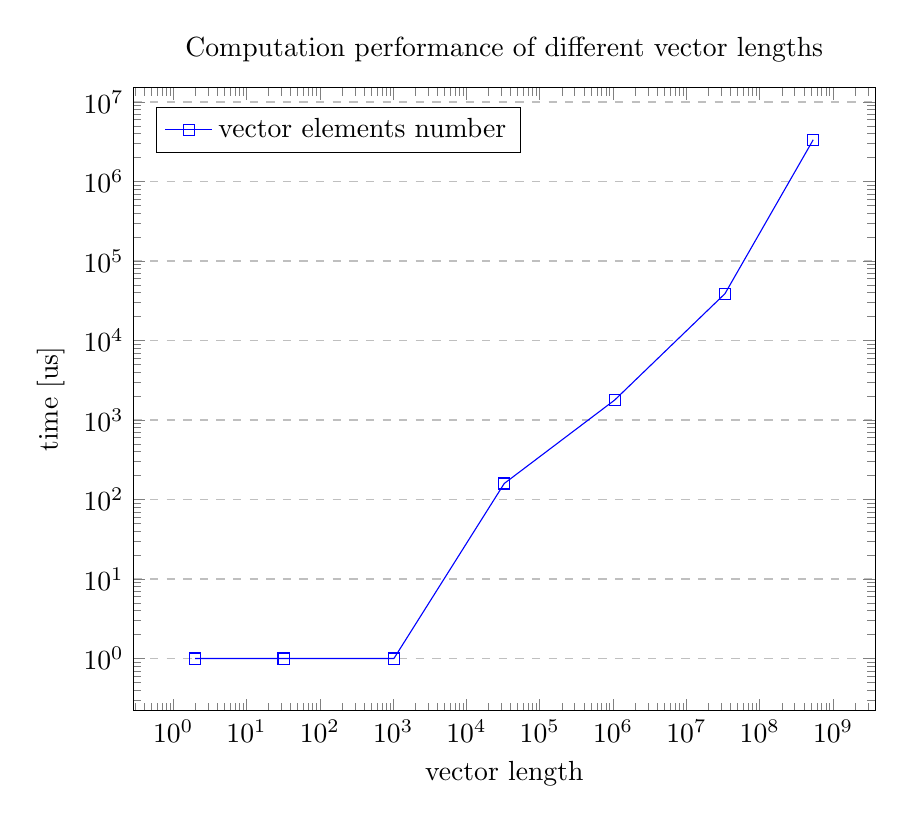
\begin{tikzpicture}
\begin{axis}[
	ymode=log,
	xmode=log,
    title={Computation performance of different vector lengths},
    xlabel={vector length},
    ylabel={time [us]},
    legend pos=north west,
    ymajorgrids=true,
    grid style=dashed,
]
 
\addplot[
    color=blue,
    mark=square,
    ]
    coordinates {
    (2,1)(2^5,1)(2^10,1)(2^15,159)(2^20,1779)(2^25,38813)(2^29,3347180)
    };
    \addlegendentry{vector elements number} 
\end{axis}
\end{tikzpicture}

A huge difference can be seen when changing data size when the size of vector is larger than the number of threads per block. When the size of vector exceeds the number of threads per block the difference of time starts to grow immediately. 

\subsection{Data transfer time comparison} \label{data_transfer}

Like in the previous experiment, first two plots present resuts for a fixed vector size $2^{27}$ and changing grid layout, where blocks and threads size are in a relation with each other in following experiments (changing thread number changes blocks number). 
\[ blocksPerGrid =  (vectorElemNumber + threadsPerBlock + 1) / threadsPerBlock \]

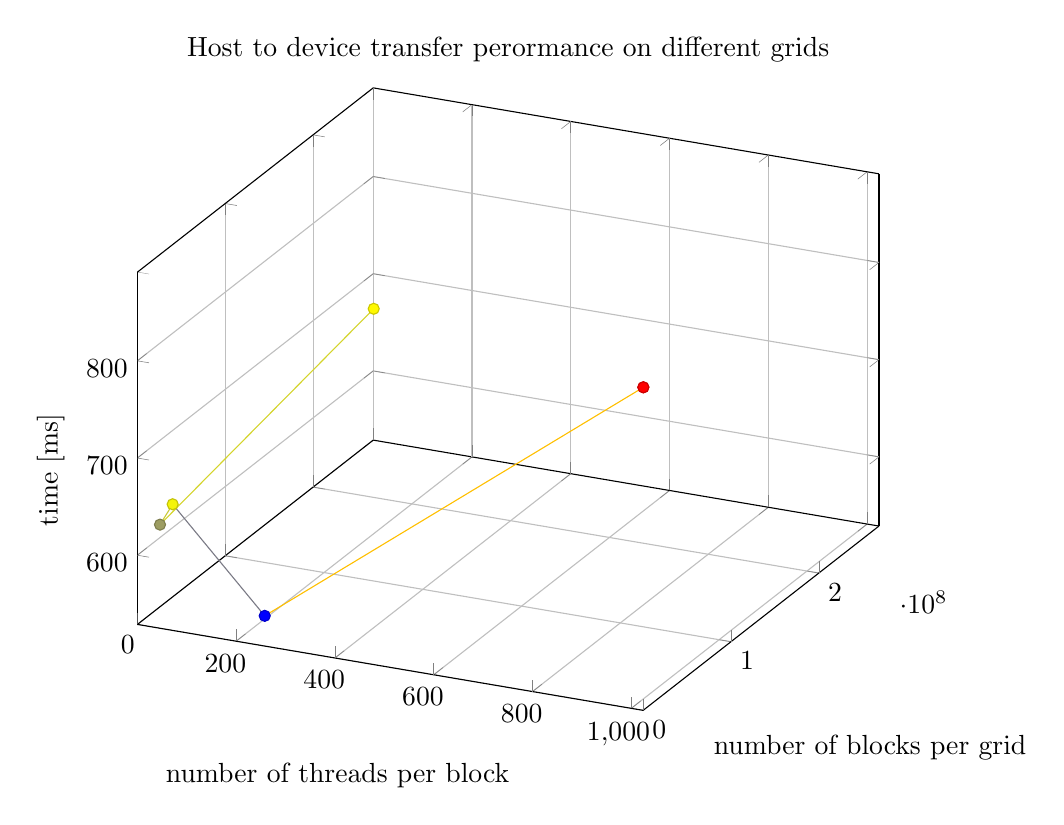
\begin{tikzpicture}
	\begin{axis}[grid=major,
	title={Host to device transfer perormance on different grids},
	xlabel={number of threads per block},
	ylabel={number of blocks per grid},
    zlabel={time [ms]},
    xmin=0, xmax=1024,
    ymin=0, ymax=268435456,
	]
	
	\addplot3+[mesh,scatter] 
		coordinates {
(1,268435456,664) (16,16777217,621) (64,4194304,655) 
(256,1048576,559) (1024,262144,861) (1024,262144,861) 
};;
	\end{axis}
\end{tikzpicture}

We can observe the best performance for grids with a lot of blocks. Those, which have high number of threads send the data for around 50\% more time. 

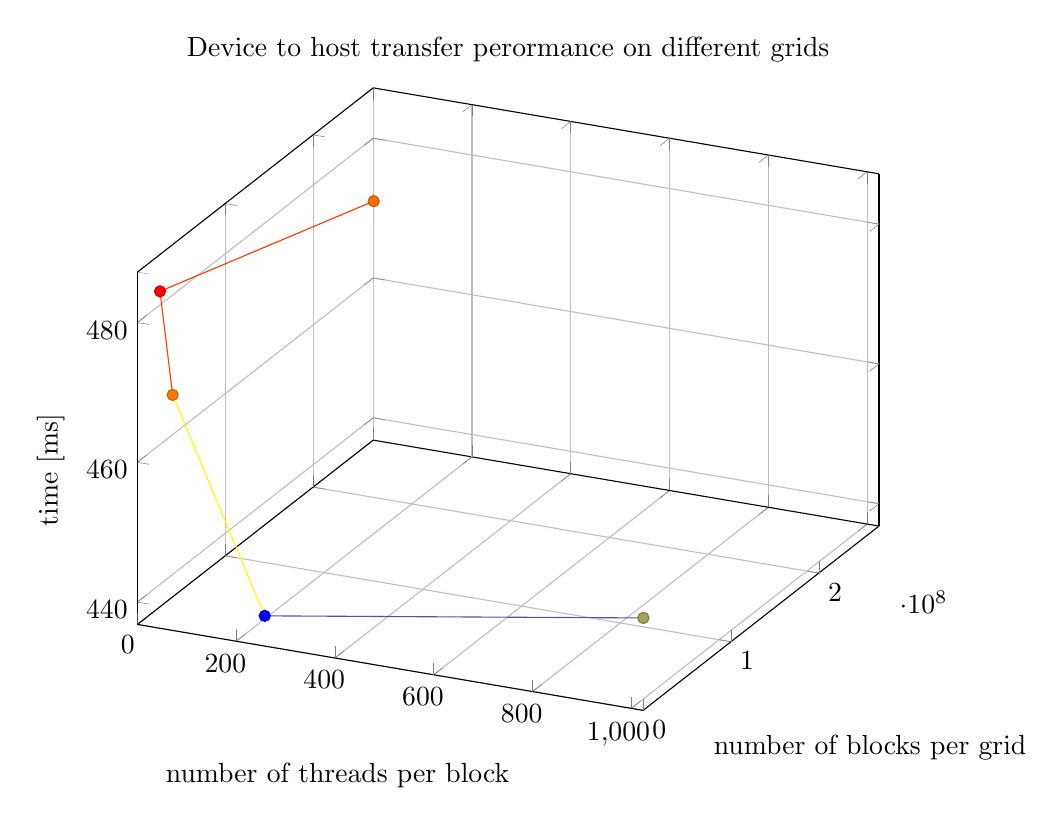
\begin{tikzpicture}
	\begin{axis}[grid=major,
	title={Device to host transfer perormance on different grids},
	xlabel={number of threads per block},
	ylabel={number of blocks per grid},
    zlabel={time [ms]},
    xmin=0, xmax=1024,
    ymin=0, ymax=268435456,
	]
	
	\addplot3+[mesh,scatter] 
		coordinates {
(1,268435456,471) (16,16777217,483) (64,4194304,470) 
(256,1048576,441) (1024,262144,450) (1024,262144,450) 
};;
	\end{axis}
\end{tikzpicture}

In the back transfer we do not observe any major differences between blocks. They are so small, that the difference can be caused by a normal timing fluctuations observed when running the same code multiple times. Based on this experiment it can be concluded that the transfer from the device to host is not affected by the size of grid in any way.

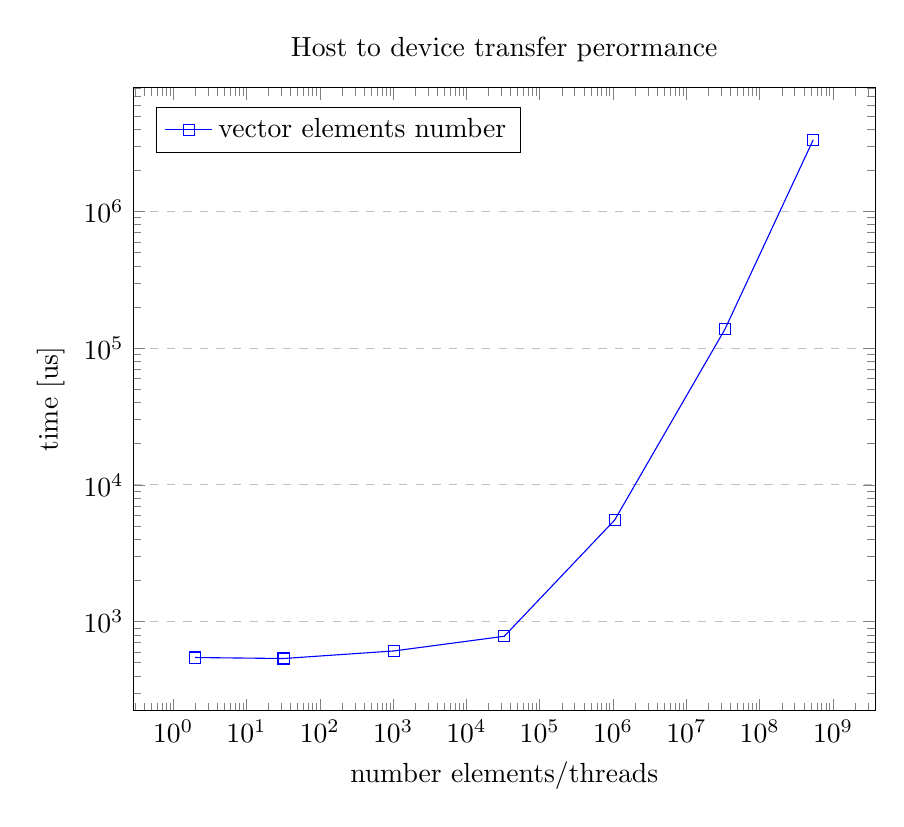
\begin{tikzpicture}
\begin{axis}[
	ymode=log,
	xmode=log,
    title={Host to device transfer perormance},
    xlabel={number elements/threads},
    ylabel={time [us]},
    legend pos=north west,
    ymajorgrids=true,
    grid style=dashed,
]
 
\addplot[
    color=blue,
    mark=square,
    ]
    coordinates {
    (2,546)(2^5,537)(2^10,610)(2^15,781)(2^20,5524)(2^25,137710)(2^29,3347180)
    };
    \addlegendentry{vector elements number} 
\end{axis}
\end{tikzpicture}

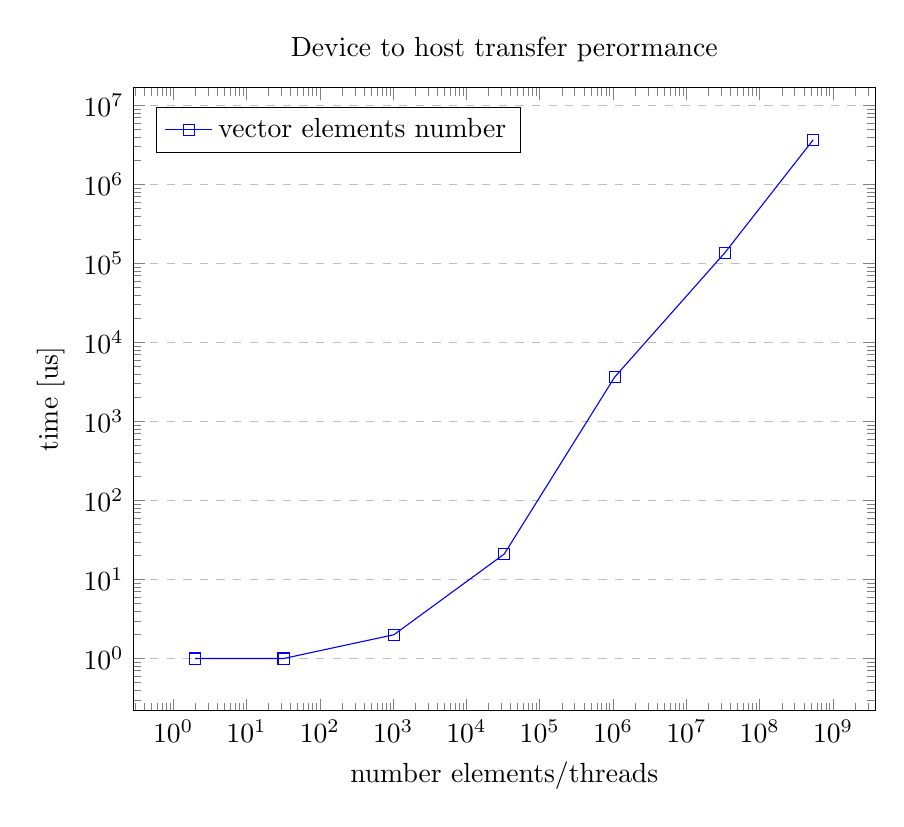
\begin{tikzpicture}
\begin{axis}[
	ymode=log,
	xmode=log,
    title={Device to host transfer perormance},
    xlabel={number elements/threads},
    ylabel={time [us]},
    legend pos=north west,
    ymajorgrids=true,
    grid style=dashed,
]
 
\addplot[
    color=blue,
    mark=square,
    ]
    coordinates {
    (2,1)(2^5,1)(2^10,2)(2^15,21)(2^20,3634)(2^25,136930)(2^29,3670480)
    };
    \addlegendentry{vector elements number}
\end{axis}
\end{tikzpicture}

In the situation of transfering we can see a very similiar behaviour to the computation one. Until the number of elements do not exceed the size of threads per grid, the transfer time is nearly freezed.

Although transfer times differ for copying from and to the device, the shape of plots look like more or less the same for both operations.

Generally, for all actions on which experiments were conucted, the time change is smaller for low figures  and bigger for high figures. It indicates, that using GPU with large number of data transfered at the same time can be less beneficial than granulating this data into subsets and processing them in small portions in GPU. That is why we should try to form our computations in group of smaller calculations, but not too small to aviod too fequent and unnecessary data copying between host and device.

\end{document}